%%####################################################################
%    Copyright @ 2007 Andreas Frieß (Friess)
%    Permission is granted to copy, distribute and/or modify this document
%    under the terms of the GNU Free Documentation License, Version 1.2
%    or any later version published by the Free Software Foundation;
%    with no Invariant Sections, no Front-Cover Texts, and no Back-Cover Texts.
%    A copy of the license is included in the section entitled ``GNU
%    Free Documentation License''.
%%####################################################################
% Created: 08.11.2007
% @cvs($Date: $)
% @cvs($Rev:  $)
% @cvs($Author: af0815 $)
% @cvs($URL: $)
%%####################################################################
\section[Data Access - Clientdatenbank Komponenten]{DataAccess}
%%####################################################################
\subsection{Beschreibung}
\subsubsection{Einleitung}
Die Komponenten auf der Seite 'Client Access' sind für die lokale\label{ClientAccess} Verwaltung von Datenbanken, auch lokale Datenbanken genannt, zuständig. \parpic[sl][r]{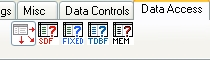
\includegraphics[width=0.3\textwidth]{Kapitel/datenbanken/pics/DataAccess}}
\label{fig:LazDataAccess01} Für die Erstellung, Verwaltung und Zugriff auf Dbase und Foxpro Datenbanken ist die Komponenete 'TDBF' zuständig. Für Datenbanken direkt im Speicher ist die Komponenete 'MEM', für Datenbanken mit eine festen Format (CSV) die Komponente 'FIXED' und Textbasierende Datensätze mittels der Komponente 'SDF'.
Für Serverdatenbanken sind die Komponenten auf der Seite 'SQLdb'\footnote{Siehe Kapitel \ref{SQLdb} auf Seite \pageref{SQLdb}} zu verwenden.

Die Komponente 'TDatasource' dient unter andern als Verbindung zu den grafischen Komponenten.

\subsection{TDatasource}

\subsection{SDF}
%  public
%    constructor Create(AOwner: TComponent); override;
%  published
%    property Delimiter: Char read FDelimiter write SetDelimiter;
%    property FirstLineAsSchema: Boolean read FFirstLineAsSchema write SetFirstLineAsSchema;
%  end;
%
\subsection{FIXED}
%  public
%    constructor Create(AOwner: TComponent); override;
%    destructor  Destroy; override;
%    function  GetFieldData(Field: TField; Buffer: Pointer): Boolean; override;
%    procedure RemoveBlankRecords; dynamic;
%    procedure RemoveExtraColumns; dynamic;
%    procedure SaveFileAs(strFileName : String); dynamic;
%    property  CanModify;
%    procedure LoadFromStream(Stream :TStream);
%    procedure SavetoStream(Stream :TStream);
%  published
%    property FileMustExist: Boolean read FFileMustExist write SetFileMustExist;
%    property ReadOnly: Boolean read FReadOnly write SetReadOnly;
%    property FileName : TFileName read FFileName write SetFileName;
%    property Schema: TStringList read FSchema write SetSchema;
%    property TrimSpace: Boolean read FTrimSpace write SetTrimSpace default True;
%    property FieldDefs;
%    property Active;
%    property AutoCalcFields;
%    property Filtered;
%    property BeforeOpen;
%    property AfterOpen;
%    property BeforeClose;
%    property AfterClose;
%    property BeforeInsert;
%    property AfterInsert;
%    property BeforeEdit;
%    property AfterEdit;
%    property BeforePost;
%    property AfterPost;
%    property BeforeCancel;
%    property AfterCancel;
%    property BeforeDelete;
%    property AfterDelete;
%    property BeforeScroll;
%    property AfterScroll;
%//    property BeforeRefresh;
%//    property AfterRefresh;
%    property OnCalcFields;
%    property OnDeleteError;
%    property OnEditError;
%    property OnFilterRecord;
%    property OnNewRecord;
%    property OnPostError;

\subsection{TDBF}

\subsection{MEM}
%\subsubsection{Datentypen}
%\begin{verbatim}
%   ftString :   result:=FieldDefs.Items[FieldNo-1].Size+1;
%   ftBoolean :  result:=SizeOf(Wordbool);
%   ftFloat :    result:=SizeOf(Double);
%   ftLargeInt : result:=SizeOf(int64);
%   ftSmallInt : result:=SizeOf(SmallInt);
%   ftInteger :  result:=SizeOf(Integer);
%   ftDate :     result:=SizeOf(TDateTime);
%   ftTime :     result:=SizeOf(TDateTime);
%   ftDateTime : result:=SizeOf(TDateTime);
%\end{verbatim}

%
%  public
%    constructor Create(AOwner:tComponent); override;
%    destructor Destroy; override;
%    procedure CreateTable;
%
%    Function  DataSize : Integer;
%
%    procedure Clear(ClearDefs : Boolean);
%    procedure Clear;
%    Procedure SaveToFile(AFileName : String);
%    Procedure SaveToFile(AFileName : String; SaveData : Boolean);
%    Procedure SaveToStream(F : TStream);
%    Procedure SaveToStream(F : TStream; SaveData : Boolean);
%    Procedure LoadFromStream(F : TStream);
%    Procedure LoadFromFile(AFileName : String);
%    Procedure CopyFromDataset(DataSet : TDataSet);
%    Procedure CopyFromDataset(DataSet : TDataSet; CopyData : Boolean);
%
%    Property Modified : Boolean Read FModified;
%
%  published
%    Property FileName : String Read FFileName Write FFileName;
%    property Filtered;
%    Property Active;
%    Property FieldDefs;
%    property BeforeOpen;
%    property AfterOpen;
%    property BeforeClose;
%    property AfterClose;
%    property BeforeInsert;
%    property AfterInsert;
%    property BeforeEdit;
%    property AfterEdit;
%    property BeforePost;
%    property AfterPost;
%    property BeforeCancel;
%    property AfterCancel;
%    property BeforeDelete;
%    property AfterDelete;
%    property BeforeScroll;
%    property AfterScroll;
%    property OnDeleteError;
%    property OnEditError;
%    property OnNewRecord;
%    property OnPostError;
%    property OnFilterRecord;
%  end;
\subsection{SQLite}
Diese Komponente ist standardmässig nicht vorhanden. Dazu muß erst das Paket 'sqlite3laz 0.3'oder besser installiert werden.  \parpic[sl][r]{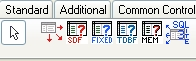
\includegraphics[width=0.3\textwidth]{Kapitel/datenbanken/pics/DataAccessLite}}
\label{fig:LazDataAccess02}Nach dem neu erstellen der IDE, befindet sich die Komponente hier.


%    function BookmarkValid(ABookmark: TBookmark): Boolean; override;
%    function CompareBookmarks(Bookmark1, Bookmark2: TBookmark): Longint; override;
%    function GetFieldData(Field: TField; Buffer: Pointer): Boolean; override;
%    function GetFieldData(Field: TField; Buffer: Pointer; NativeFormat: Boolean): Boolean; override;
%    function Locate(const KeyFields: string; const KeyValues: Variant; Options: TLocateOptions) : Boolean; override;
%    function LocateNext(const KeyFields: string; const KeyValues: Variant; Options: TLocateOptions) : Boolean;
%    function Lookup(const KeyFields: string; const KeyValues: Variant; const ResultFields: string): Variant;override;
%    // Additional procedures
%    function ApplyUpdates: Boolean;
%    function CreateTable: Boolean;
%    function CreateTable(const ATableName: String): Boolean;
%    procedure ExecCallback(const ASql: String; UserData: Pointer = nil);
%    procedure ExecSQLList;
%    procedure ExecuteDirect(const ASql: String);virtual;abstract;
%    procedure QueryUpdates(RecordStates: TRecordStateSet; Callback: TQueryUpdatesCallback; UserData: Pointer=nil);
%    function QuickQuery(const ASql:String):String;overload;
%    function QuickQuery(const ASql:String;const AStrList: TStrings):String;overload;
%    function QuickQuery(const ASql:String;const AStrList: TStrings;FillObjects:Boolean):String;virtual;abstract;overload;
%    procedure RefetchData;
%    function TableExists: Boolean;
%    function TableExists(const ATableName:String):Boolean;
%    function UpdatesPending: Boolean;
%    property ExpectedAppends: Integer read FExpectedAppends write SetExpectedAppends;
%    property ExpectedUpdates: Integer read FExpectedUpdates write SetExpectedUpdates;
%    property ExpectedDeletes: Integer read FExpectedDeletes write SetExpectedDeletes;
%    property IndexFields[Value: Integer]: TField read GetIndexFields;
%    property RowsAffected: Integer read GetRowsAffected;
%    property ReturnCode: Integer read FReturnCode;
%    property SqliteHandle: Pointer read FSqliteHandle;
%    property SqliteVersion: String read GetSqliteVersion;
%    property SQLList:TStrings read FSqlList;
%   published
%    property AutoIncrementKey: Boolean read FAutoIncrementKey write FAutoIncrementKey;
%    property IndexFieldNames: string read FIndexFieldNames write FIndexFieldNames;
%    property FileName: String read FFileName write SetFileName;
%    property OnCallback: TSqliteCallback read FOnCallback write FOnCallback;
%    property PrimaryKey: String read FPrimaryKey write FPrimaryKey;
%    
%    property TableName: String read FTableName write FTableName;   
%    property MasterSource: TDataSource read GetMasterSource write SetMasterSource;
%    property MasterFields: string read GetMasterFields write SetMasterFields;
%    
\subsubsection{ExecSQL}
\begin{description}
  \item \texttt{procedure ExecSQL(const ASql:String);}\\Führt den in ASql definierten String aus, liefert aber keine Datenmenge zurück.
  \item \texttt{procedure ExecSQL;}\\Führt die in der Eigenschaft SQL definierten SQL-Befehle aus, liefert aber keine Datenmenge zurück.
  \begin{description}
    \item Methode von TSqlite3Dataset
  \end{description}
\end{description}

\subsubsection{ApplyUpdates}
\begin{description}
  \item \texttt{function ApplyUpdates: Boolean;}\\Überträgt die Änderungen von der Datenmenge in die Datenbank.
  \begin{description}
    \item Methode von TSqlite3Dataset>TCustomSqliteDataset
  \end{description}
\end{description}

\subsubsection{ExecSQL}
\begin{description}
  \item \texttt{procedure ExecSQL(const ASql:String);}\\Führt den in ASql definierten String aus, liefert aber keine Datenmenge zurück.
  \item \texttt{procedure ExecSQL;}\\Führt die in der Eigenschaft SQL definierten SQL-Befehle aus, liefert aber keine Datenmenge zurück.
  \begin{description}
    \item Methode von TSqlite3Dataset
  \end{description}
\end{description}

\subsubsection{Active}
\begin{description}
  \item \texttt{property Active: Boolean read GetActive write SetActive default False;}\\ Sagt aus ob die Komponente derzeit aktiv ist und eine Datenmenge zurückliefert. Ein setzen auf 'true' entspricht der Methode 'Open' und ein setzen auf 'false' entspricht der Methode 'Close'.
  \begin{description}
    \item Eigenschaft von TSqlite3Dataset>TCustomSqliteDataset>TDataSet
  \end{description}
  \begin{description}
    \item Zugriff: Lesend und schreibend
    \item Defaultwert: false
  \end{description}
\end{description}

\subsubsection{SaveOnClose}
\begin{description}
  \item \texttt{property SaveOnClose: Boolean read FSaveOnClose write FSaveOnClose;}\\Wenn true, dann wird beim Schliessen der Datenmenge automatisch ein ApplyUpdates durchgeführt.
  \begin{description}
    \item Eigenschaft von TSqlite3Dataset>TCustomSqliteDataset
  \end{description}
  \begin{description}
    \item Zugriff: Lesend und schreibend
  \end{description}
\end{description}

\subsubsection{SaveOnRefetch}
\begin{description}
  \item \texttt{property SaveOnRefetch: Boolean read FSaveOnRefetch write FSaveOnRefetch;}\\Wenn true, dann wird vor dem Holen neuer Datenmengen automatisch ein ApplyUpdates durchgeführt.
  \begin{description}
    \item Eigenschaft von TSqlite3Dataset>TCustomSqliteDataset
  \end{description}
  \begin{description}
    \item Zugriff: Lesend und schreibend
  \end{description}
\end{description}

\subsubsection{SQL}
\begin{description}
  \item \texttt{property SQL: String read FSql write FSql;}\\In SQL befindet sich das SQL Statement was ausgeführt werden soll.
  \begin{description}
    \item Eigenschaft von TSqlite3Dataset>TCustomSqliteDataset
  \end{description}
  \begin{description}
    \item Zugriff: Lesend und schreibend
  \end{description}
\end{description}

\verb|Version: $$ |\footnote{ Autor: Andreas Frieß\\Lizenz: GFDL}